% Preamble
\documentclass[12pt,a4paper]{article}
\usepackage{enumerate} 	
\usepackage{setspace}						
\usepackage{authblk}	
\usepackage{graphicx} 	
%\usepackage[nomarkers, nolists]{endfloat} 
\usepackage{pdflscape}	
\usepackage{mathtools}	
\usepackage[osf]{mathpazo} 
\usepackage{lineno} 	
\usepackage{hyperref}
\usepackage[round]{natbib} 
\usepackage{setspace}

\setcounter{secnumdepth}{0} 
\raggedright 			
\pagenumbering{arabic}	

\renewcommand{\thetable}{A\arabic{table}}
\renewcommand{\thefigure}{A\arabic{figure}}

% First order headings upper case bold
\usepackage{titlesec}
\titleformat*{\section}{\small\bfseries\uppercase}

% Second order headings normal case italics
\titleformat*{\subsection}{\small\itshape}

% Third order, italics, paragraph style
\titleformat*{\paragraph}{\small\itshape}

\begin{document}

\noindent{\Large \bf Supporting Information from `Time for a rethink: time sub-sampling methods in disparity-through-time analyses'}

\raggedright
\setlength{\parindent}{1cm}

\section{Appendix S1: Extra details of datasets}

\subsection{Beck2014 (Figure \ref{figure:beck})}
The following taxa were removed because they were in the phylogeny but not the character matrix or vice versa: \textit{Montanalestes}, \textit{Lainodon}, \textit{Kharmerungulatum}, \textit{Alymlestes}. 

\subsection{Brusatte2014 (Figure \ref{figure:brusatte})} 
We used one randomly selected time-scaled tree from Brusatte et al. (2014).
Zero-length branches were replaced with the minimum branch length in the phylogeny.
The following taxa were removed because they were in the phylogeny but not the character matrix or vice versa: \textit{Sinraptor dongi}, \textit{Hesperonychus elizabethae}, \textit{Pyroraptor olympius}, \textit{Limenavis patagonica}, \textit{Lithornis}, \textit{Crypturellus undulatus}, \textit{Gallus gallus}, \textit{Crax pauxi}, \textit{Anas platyrhynchus}, \textit{Chauna torquata}, \textit{Epidendrosaurus} and \textit{Kinnareemimus}. 
The following taxa were removed because they shared no characters in the morphological matrix: \textit{Shanag ashile}, \textit{Atrociraptor marshalli}, \textit{Proceratosaurus bradleyi}, \textit{Incisivosaurus gauthieri}, \textit{Enigmosaurus}, \textit{Nanshiungosaurus brevispinus}, \textit{Xixiasaurus}, \textit{Tsaagan mangas}, \textit{Mirischia}, \textit{Pedopenna}, \textit{Suzhousaurus}, \textit{Juratyrant}, \textit{Vorona}, \textit{Bonapartenykus}, \textit{Teratophoneus}, \textit{Gobipteryx}, \textit{Songlingornis}, \textit{Liaoningornis longidigitu} and \textit{Achillesaurus}.   

\subsection{Bapst2016 (Figure \ref{figure:bapst})} 
We used the maximum clade credibility tree from Bapst et al. (2016).
Zero-length branches were replaced with the minimum branch length in the phylogeny.
The following taxa were removed because they were in the phylogeny but not the character matrix or vice versa: \textit{Mei long} and \textit{Mei lon}. 
The following taxa were removed because they shared no characters in the morphological matrix: \textit{Hagryphus giganteus}, \textit{Atrociraptor marshalli}, \textit{IGM100 1015 UndesDromaeosaurid}, \textit{Dromaeosaurus albertensis}, \textit{Incisivosaurus gauthieri}, \textit{Deinocheirus mirificus}, \textit{Therizinosaurus cheloniformis},  \textit{Anserimimus planinychus} and \textit{Elmisaurus rarus}. 

\subsection{Wright2017 (Figure \ref{figure:wright})}
We used the maximum clade credibility tree from Wright (2017). 
To properly timescale the tree we followed the advice of Wright (2017) and divided the branch lengths by the corresponding clock rate (= 0.03517385)  and then set the root time to 485.4. 
Zero-length branches were replaced with the minimum branch length in the phylogeny.
No taxa were removed. 

\begin{figure}[!htbp]
    \centering
    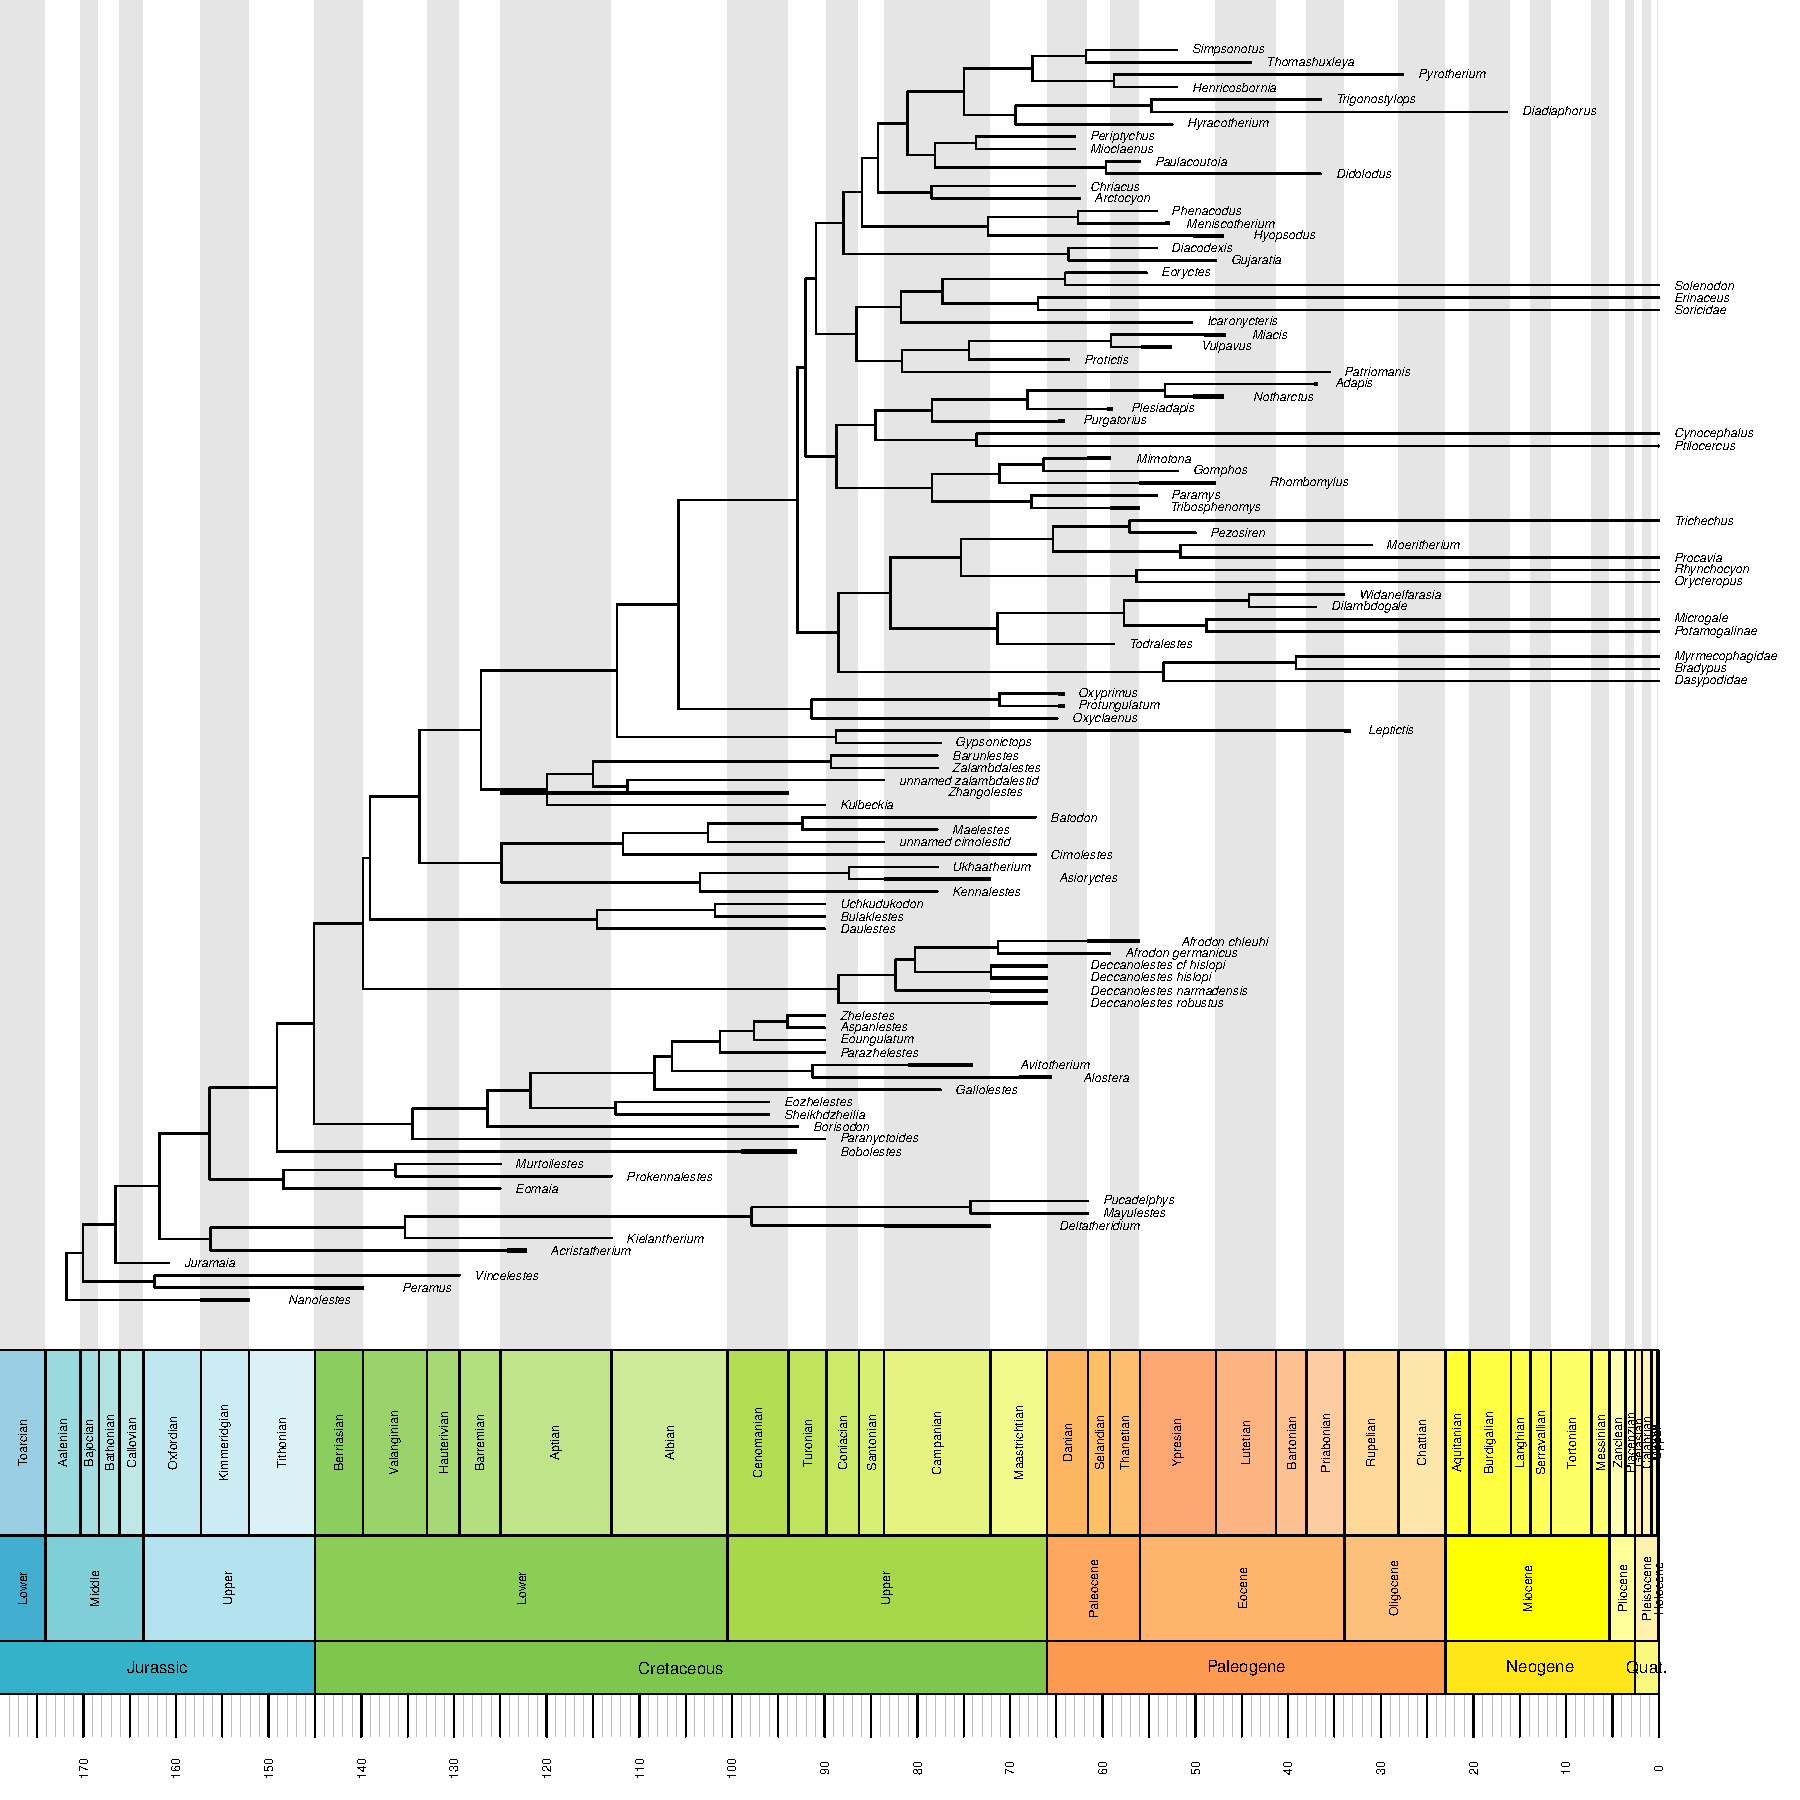
\includegraphics[width=1\linewidth, height=1\textheight, keepaspectratio]{figures/fig-tree-Beck2014-appendix.pdf}
    \caption[Beck2014.]
    {Phylogeny from Beck \& Lee (2014).}
    \label{figure:beck}
  \end{figure} 

\begin{figure}[!htbp]
    \centering
    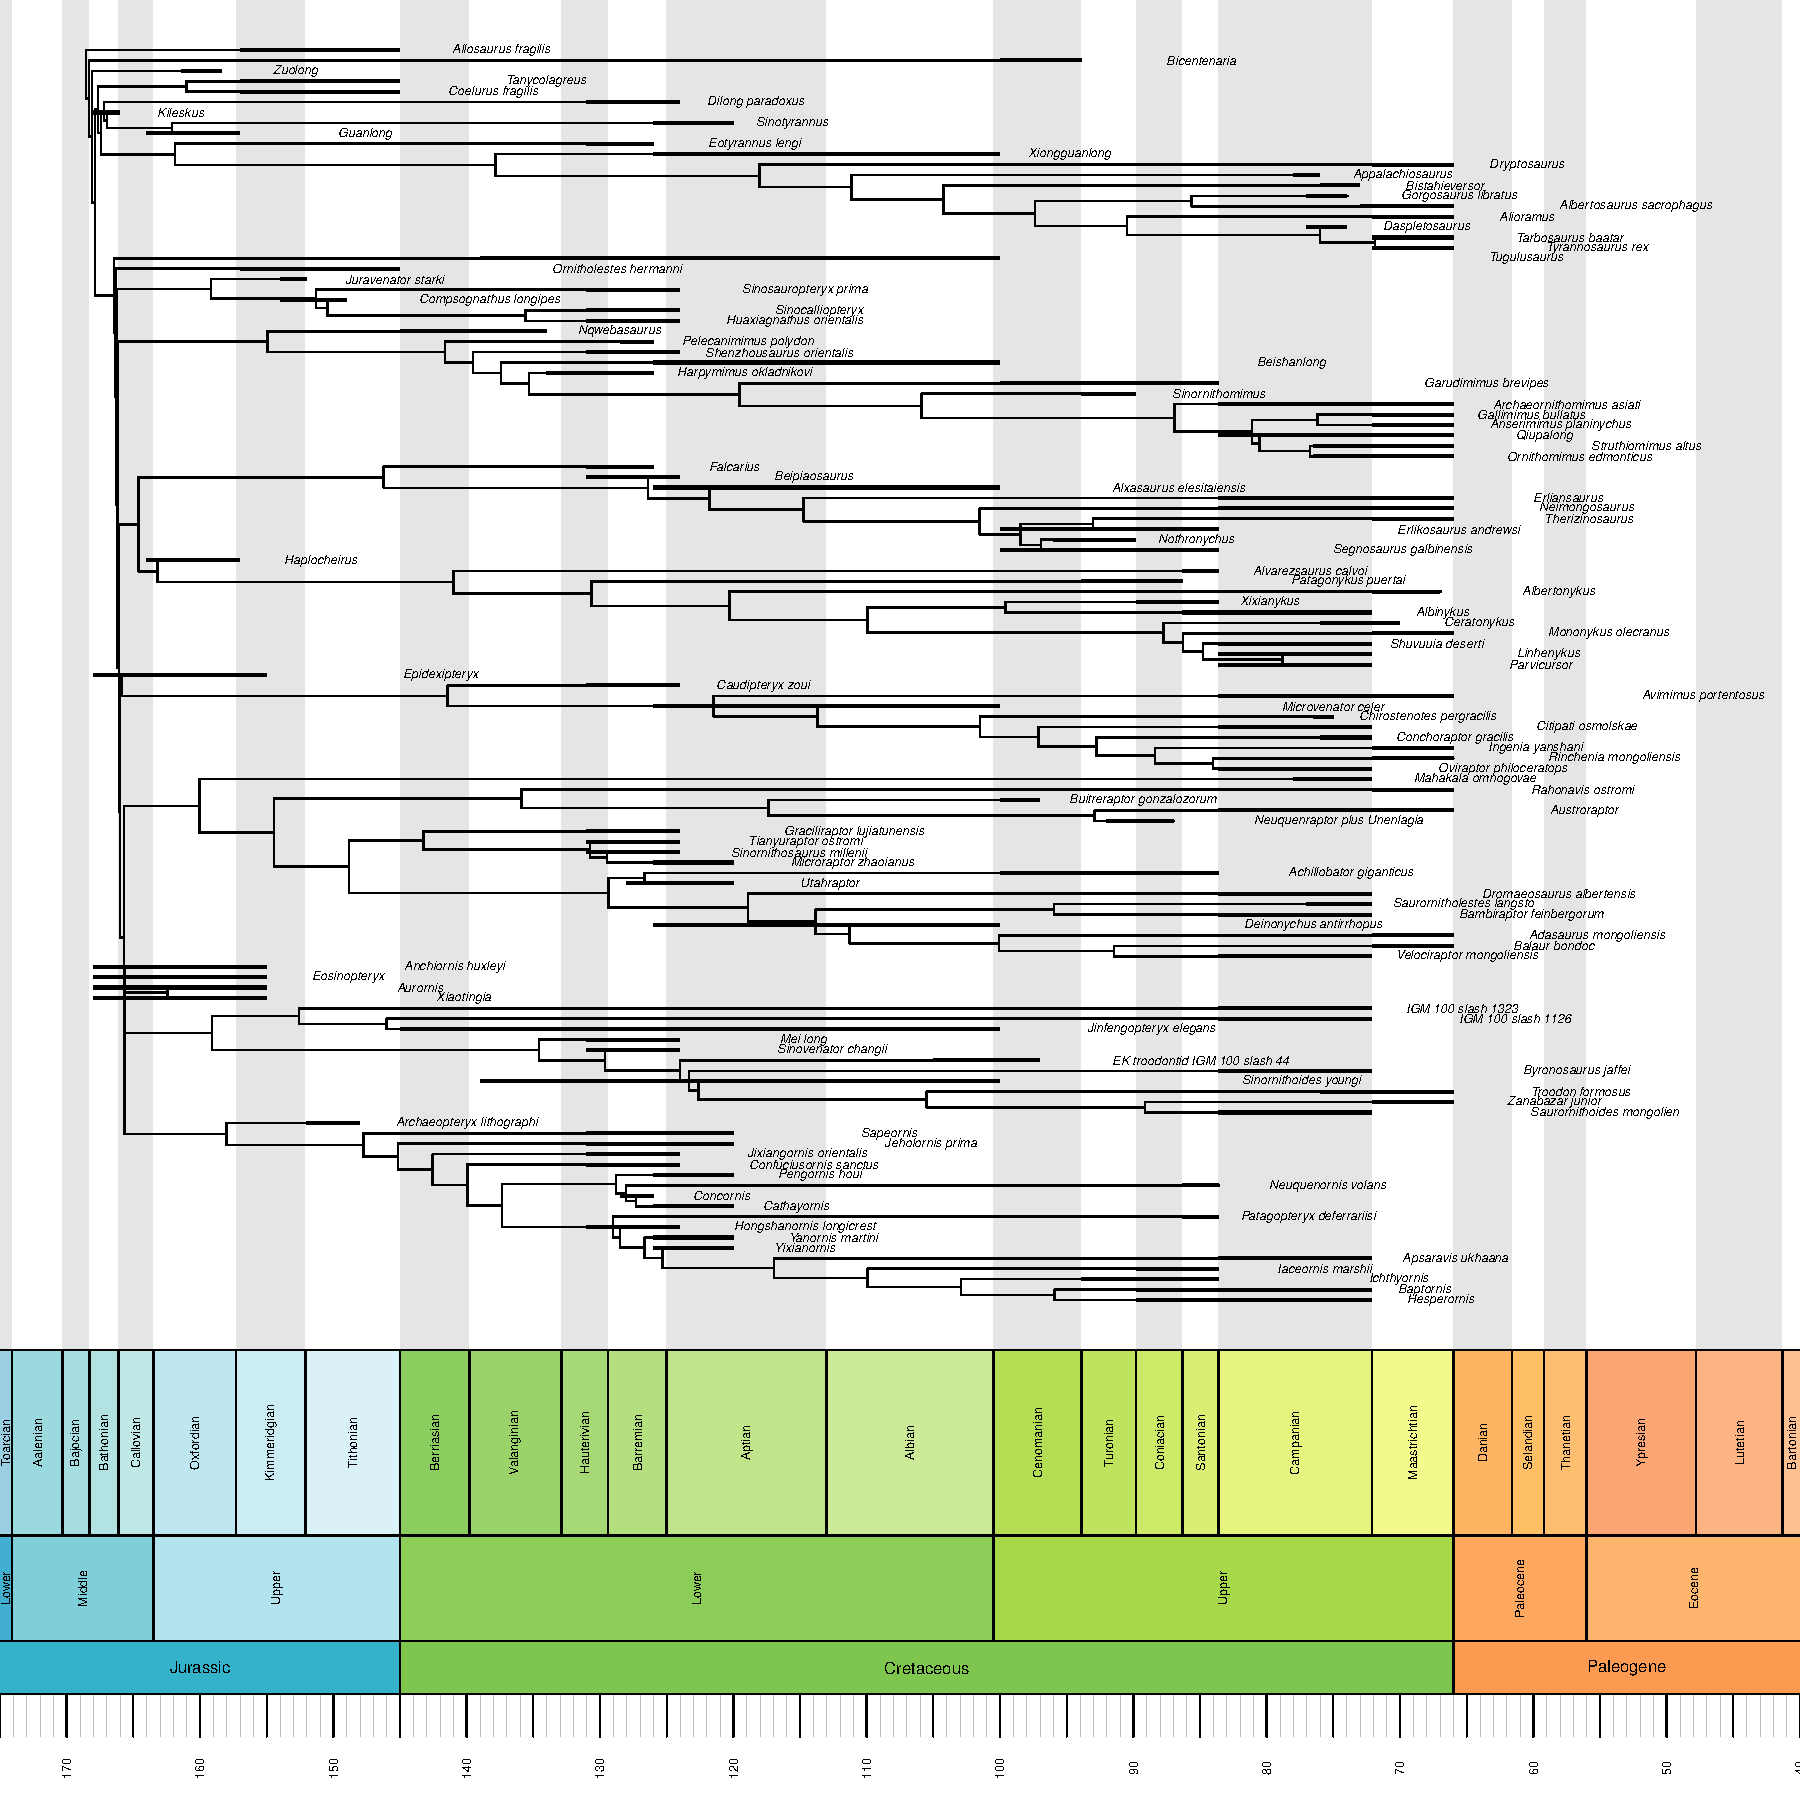
\includegraphics[width=1\linewidth, height=1\textheight, keepaspectratio]{figures/fig-tree-Brusatte2014-appendix.pdf}
    \caption[Brusatte2014.]
    {Phylogeny from Brusatte et al. (2014). This is one randomly selected tree from the time-scaled trees in the paper.}
    \label{figure:brusatte}
  \end{figure} 

\begin{figure}[!htbp]
    \centering
    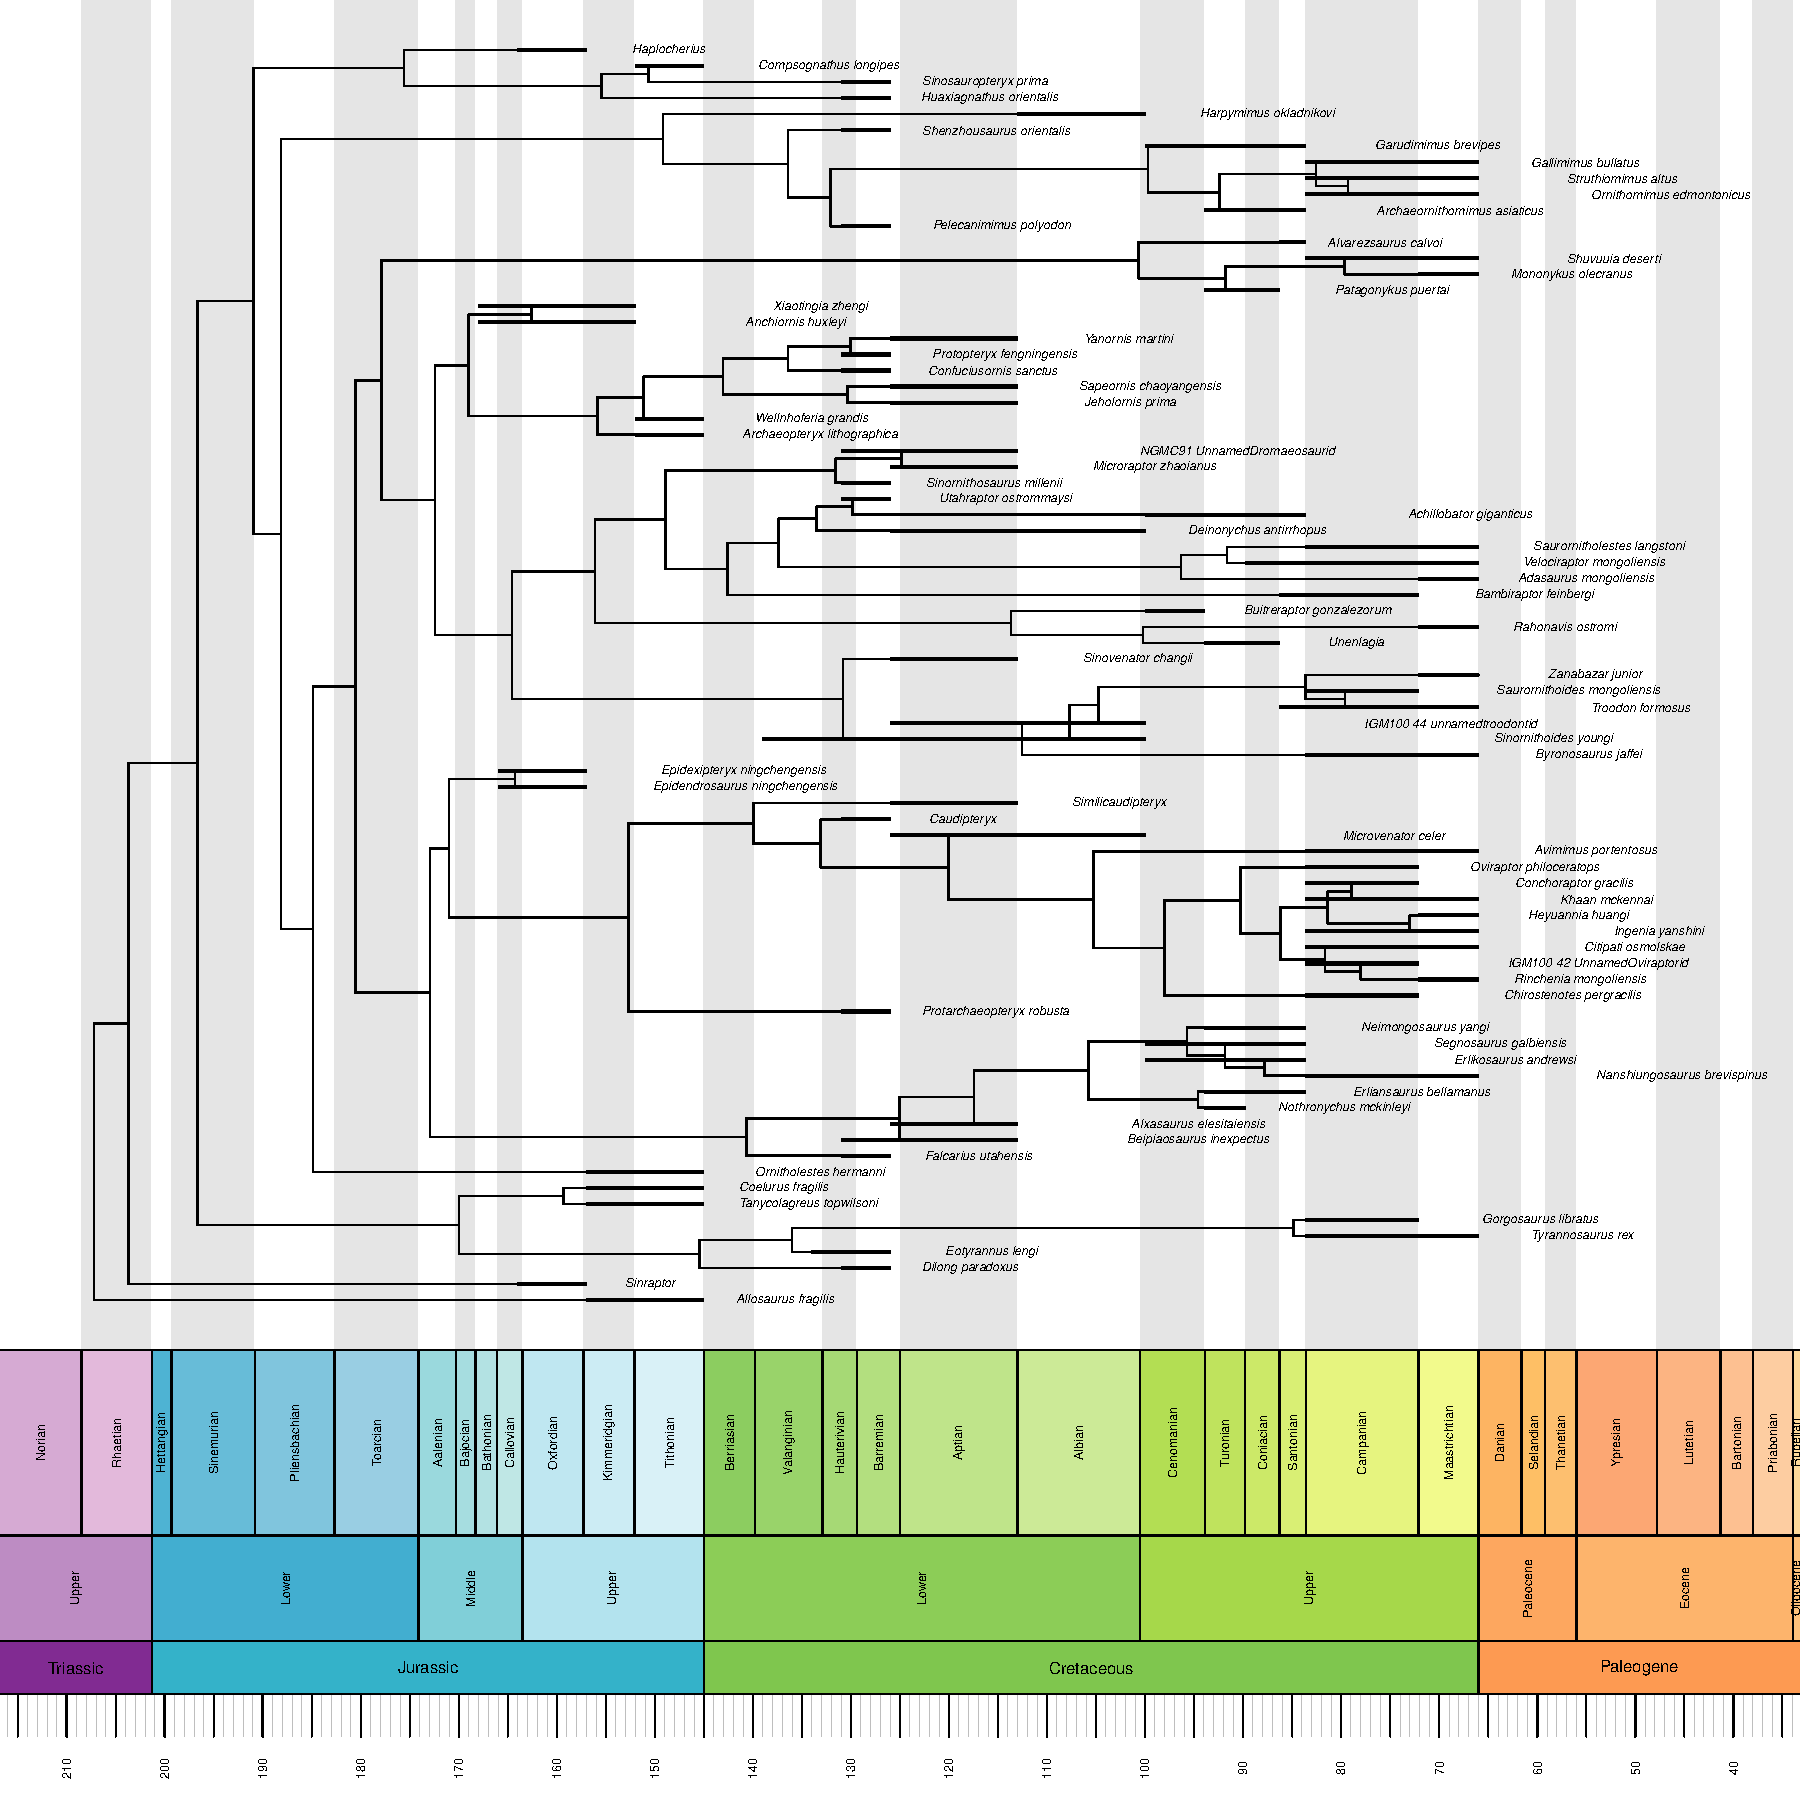
\includegraphics[width=1\linewidth, height=1\textheight, keepaspectratio]{figures/fig-tree-Bapst2016-appendix.pdf}
    \caption[Bapst2016.]
    {Phylogeny from Bapst et al. (2016). This is the maximum clade credibility tree.}
    \label{figure:bapst}
  \end{figure} 

\begin{figure}[!htbp]
    \centering
    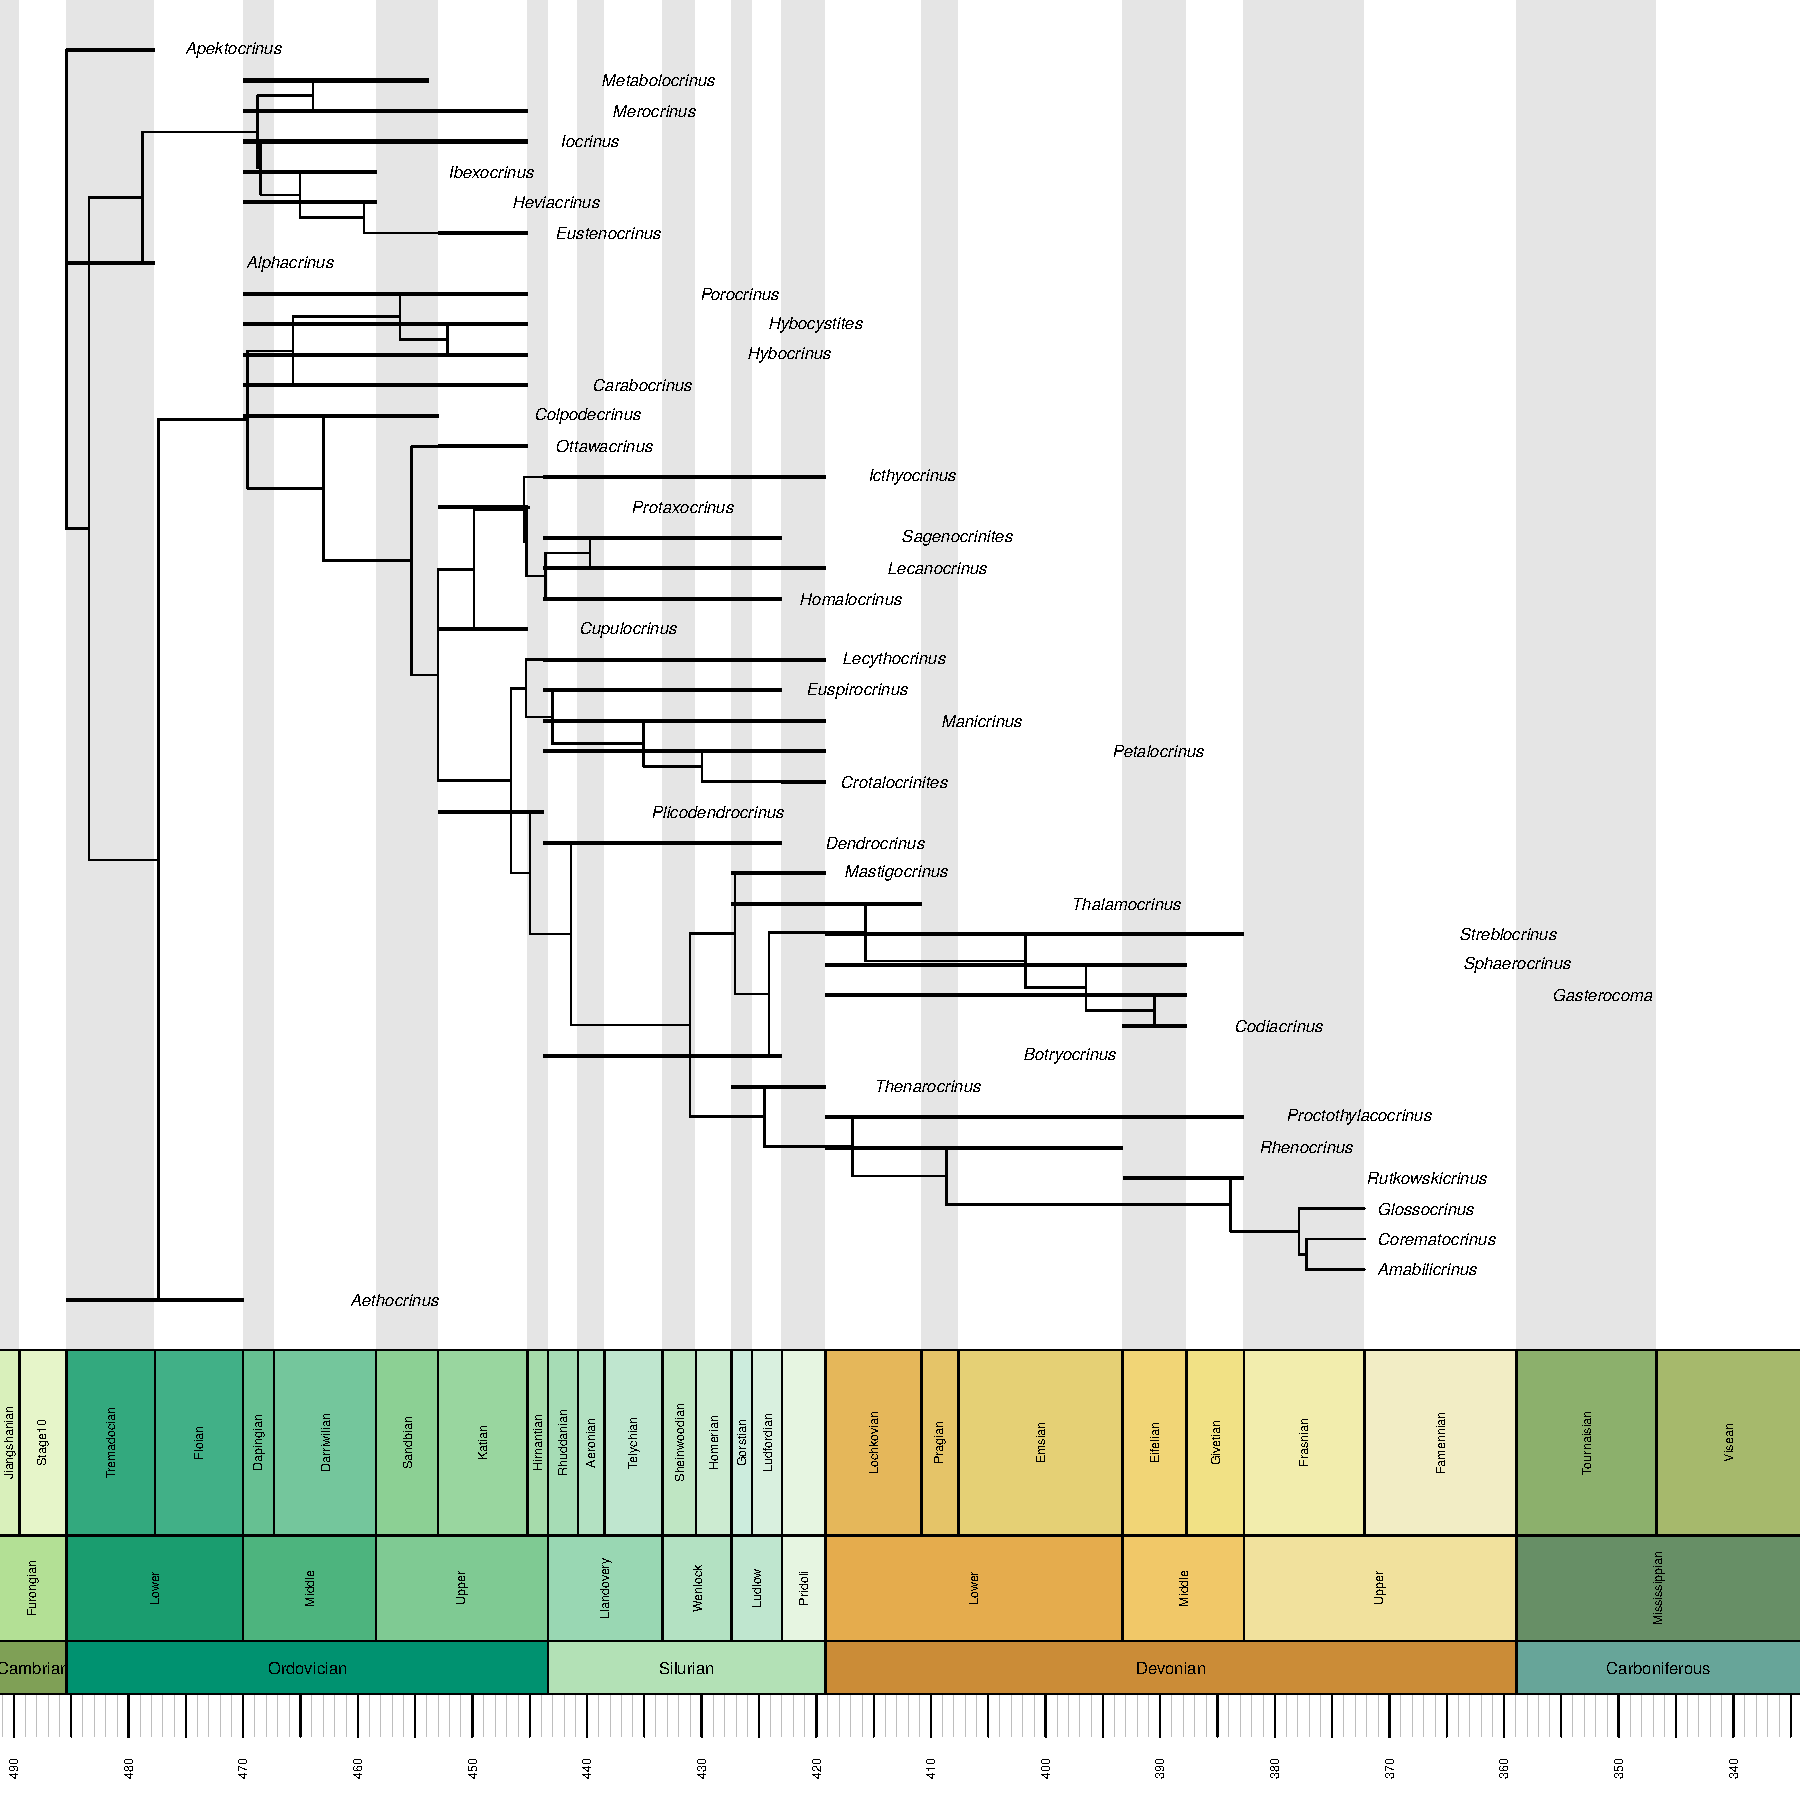
\includegraphics[width=1\linewidth, height=1\textheight, keepaspectratio]{figures/fig-tree-Wright2017-appendix.pdf}
    \caption[Wright2017.]
    {This is the maximum clade credibility tree from Wright (2017).}
    \label{figure:wright}
  \end{figure}  

\newpage
\section{Appendix S2: Additional tables and figures}

% DTT figures
  \begin{figure}[!htbp]
    \centering
    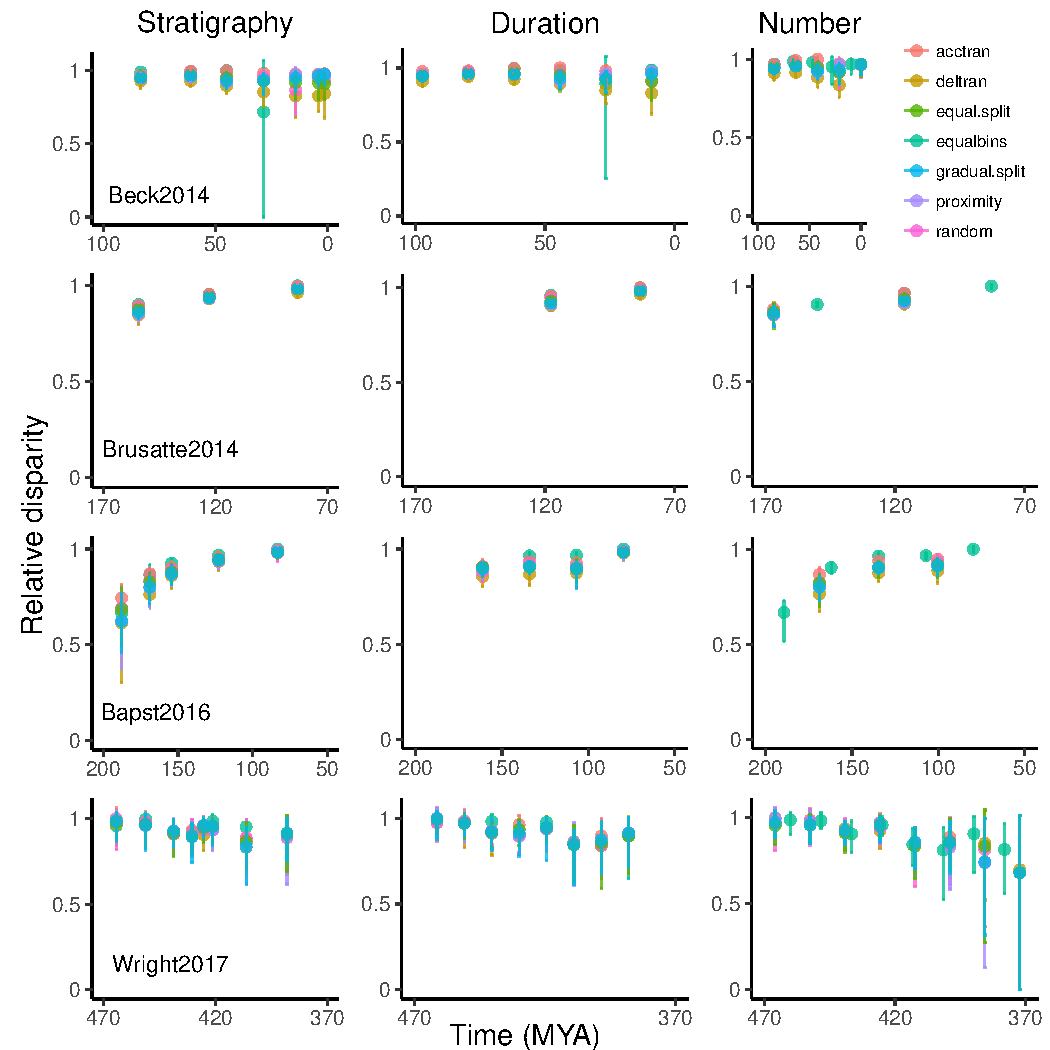
\includegraphics[width=1\linewidth, height=1\textheight, keepaspectratio]{figures/fig-dtt-epoch-appendix.pdf}
    \caption[Relative disparity through time for four example datasets.]
    {Median bootstrapped disparities were calculated using time binning and time-slicing approaches. 
    Relative disparities (median bootstrapped disparity divided by the maximum median bootstrapped disparity for a dataset and analysis method) are presented so they can be compared across datasets/methods. 
    Stratigraphy uses unequal time bins or non-equidistant slices, where the width of the bin, or the interval between slices, is equivalent to stratigraphic epochs. 
    Duration uses equal time bins or equidistant slices, where the width of the bin, or the interval between slices, is the average duration of stratigraphic epochs in the time frame of the dataset. 
    Number uses equal time bins or equidistant slices, where the number of bins, or the number of slices, is the average number of stratigraphic epochs in the time frame of the dataset. 
    In all cases, time bin disparities are plotted at the midpoint of the bin, and error bars represent the 95\% confidence intervals around the bootstrapped median disparity.
    The four dataset names are on the first plot for each dataset (Table \ref{table:datasets}).}
    \label{figure:dtt2}
  \end{figure}  

  \begin{figure}[!htbp]
    \centering
    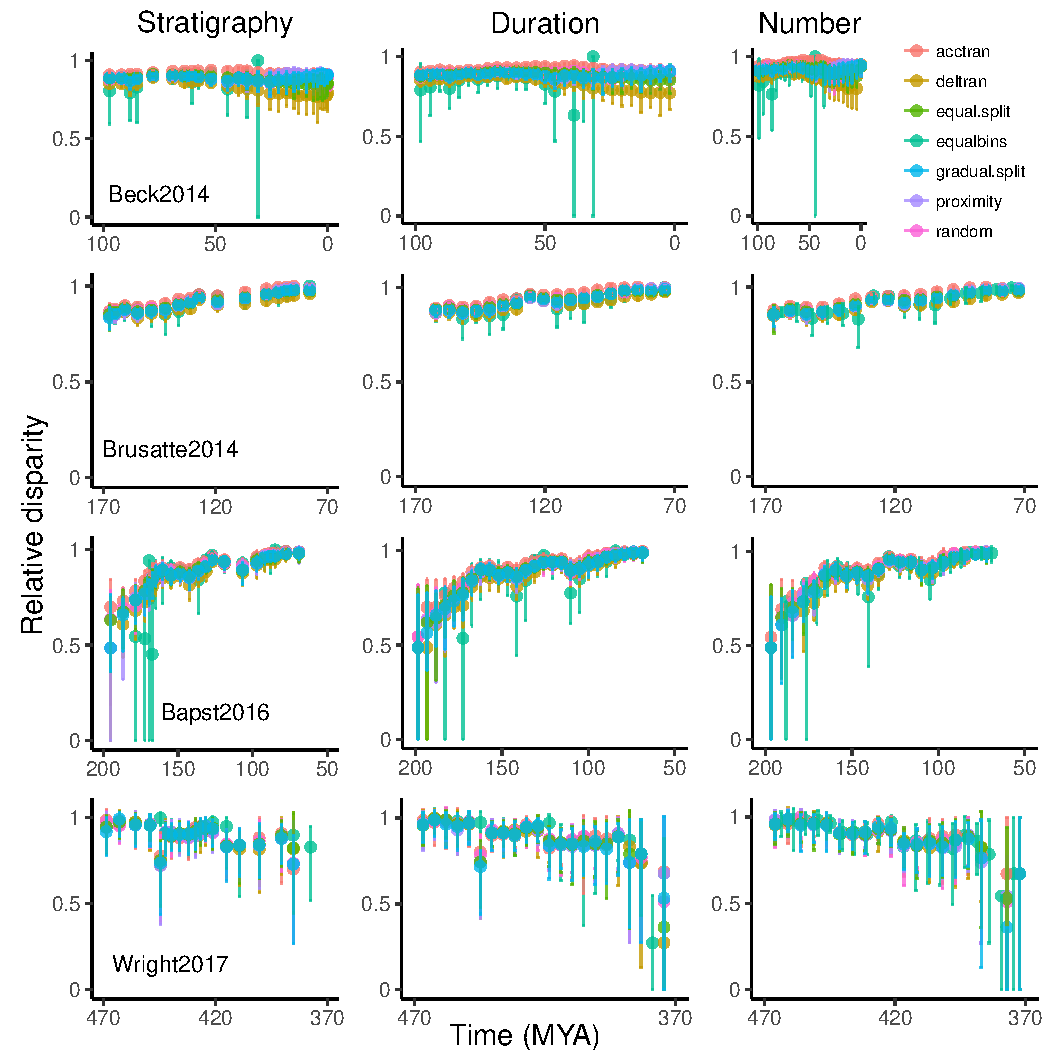
\includegraphics[width=1\linewidth, height=1\textheight, keepaspectratio]{figures/fig-dtt-age-appendix.pdf}
    \caption[Relative disparity through time for four example datasets.]
    {Median bootstrapped disparities were calculated using time binning and time-slicing approaches. 
    Relative disparities (median bootstrapped disparity divided by the maximum median bootstrapped disparity for a dataset and analysis method) are presented so they can be compared across datasets/methods. 
    Stratigraphy uses unequal time bins or non-equidistant slices, where the width of the bin, or the interval between slices, is equivalent to stratigraphic ages. 
    Duration uses equal time bins or equidistant slices, where the width of the bin, or the interval between slices, is the average duration of stratigraphic ages in the time frame of the dataset. 
    Number uses equal time bins or equidistant slices, where the number of bins, or the number of slices, is the average number of stratigraphic ages in the time frame of the dataset. 
    In all cases, time bin disparities are plotted at the midpoint of the bin, and error bars represent the 95\% confidence intervals around the bootstrapped median disparity.
    The four dataset names are on the first plot for each dataset (Table \ref{table:datasets}).}
    \label{figure:dtt3}
  \end{figure}  

% Wilcoxon results table
  % latex table generated in R 3.4.2 by xtable 1.8-2 package
% Fri Dec  8 17:06:33 2017
\begin{table}[!htbp]
\centering
\begin{tabular}{lllccc}
  \hline
\textbf{Dataset} & \textbf{Period} & \textbf{Model} & \textbf{Stratigraphy} & \textbf{Duration} & \textbf{Number} \\ 
  \hline
Beck2014 & Age & acctran & 39*** & 76 & 11 \\ 
  Beck2014 & Age & deltran & 188*** & 194*** & 171 \\ 
  Beck2014 & Age & equal.split & 91 & 119*** & 47 \\ 
  Beck2014 & Age & gradual.split & 111 & 115*** & 65*** \\ 
  Beck2014 & Age & proximity & 105 & 83 & 68*** \\ 
  Beck2014 & Age & random & 97 & 104*** & 45 \\ 
  Beck2014 & Epoch & acctran & 14 & 10 & 14 \\ 
  Beck2014 & Epoch & deltran & 21 & 45*** & 41*** \\ 
  Beck2014 & Epoch & equal.split & 21 & 40*** & 42*** \\ 
  Beck2014 & Epoch & gradual.split & 21 & 39 & 43*** \\ 
  Beck2014 & Epoch & proximity & 21 & 36 & 32 \\ 
  Beck2014 & Epoch & random & 21 & 37 & 45*** \\ 
  Brusatte2014 & Age & acctran & 27*** & 28 & 28*** \\ 
  Brusatte2014 & Age & deltran & 27*** & 29 & 31*** \\ 
  Brusatte2014 & Age & equal.split & 28*** & 58*** & 50*** \\ 
  Brusatte2014 & Age & gradual.split & 28*** & 61*** & 52*** \\ 
  Brusatte2014 & Age & proximity & 27*** & 31 & 28*** \\ 
  Brusatte2014 & Age & random & 27*** & 27 & 27*** \\ 
  Brusatte2014 & Epoch & acctran & 0 & 5*** & 5 \\ 
  Brusatte2014 & Epoch & deltran & 0 & 5*** & 5 \\ 
  Brusatte2014 & Epoch & equal.split & 3 & 6 & 6 \\ 
  Brusatte2014 & Epoch & gradual.split & 3 & 6 & 6 \\ 
  Brusatte2014 & Epoch & proximity & 0 & 5*** & 5 \\ 
  Brusatte2014 & Epoch & random & 0 & 5*** & 5 \\ 
  Bapst2016 & Age & acctran & 45*** & 47 & 72*** \\ 
  Bapst2016 & Age & deltran & 55*** & 46 & 78*** \\ 
  Bapst2016 & Age & equal.split & 93 & 147*** & 153 \\ 
  Bapst2016 & Age & gradual.split & 93 & 153 & 165 \\ 
  Bapst2016 & Age & proximity & 57*** & 47 & 75*** \\ 
  Bapst2016 & Age & random & 57*** & 48 & 81*** \\ 
  Bapst2016 & Epoch & acctran & 2 & 0*** & 8 \\ 
  Bapst2016 & Epoch & deltran & 2 & 0*** & 9 \\ 
  Bapst2016 & Epoch & equal.split & 4 & 6 & 13 \\ 
  Bapst2016 & Epoch & gradual.split & 4 & 6 & 12 \\ 
  Bapst2016 & Epoch & proximity & 2 & 0*** & 8 \\ 
  Bapst2016 & Epoch & random & 2 & 1*** & 8 \\ 
  Wright2017 & Age & acctran & 146*** & 146 & 84 \\ 
  Wright2017 & Age & deltran & 162*** & 138 & 101 \\ 
  Wright2017 & Age & equal.split & 151*** & 160 & 105 \\ 
  Wright2017 & Age & gradual.split & 152*** & 155 & 116 \\ 
  Wright2017 & Age & proximity & 160*** & 175*** & 101 \\ 
  Wright2017 & Age & random & 150*** & 147 & 111 \\ 
  Wright2017 & Epoch & acctran & 25 & 20 & 18 \\ 
  Wright2017 & Epoch & deltran & 27 & 26 & 25 \\ 
  Wright2017 & Epoch & equal.split & 29 & 30 & 25 \\ 
  Wright2017 & Epoch & gradual.split & 28 & 29 & 21 \\ 
  Wright2017 & Epoch & proximity & 23 & 28 & 18 \\ 
  Wright2017 & Epoch & random & 28 & 23 & 17 \\ 
   \hline
\end{tabular}
\caption{Wilcoxon results for appendix} 
\end{table}
 
  \label{table:wilcox2}  

% disparity peaks figures
\begin{figure}[!htbp]
    \centering
    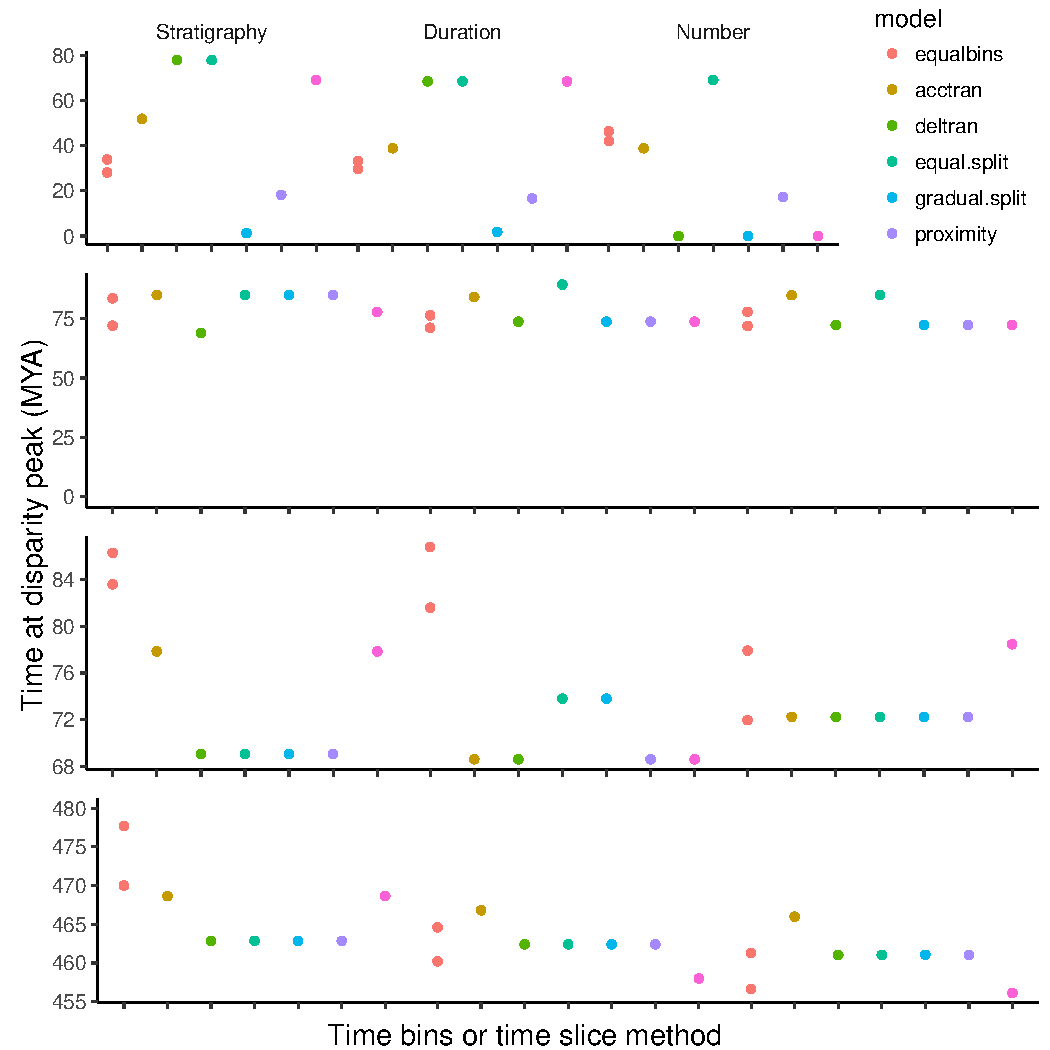
\includegraphics[width=1\linewidth, height=1\textheight, keepaspectratio]{figures/fig-peaks-epoch-appendix.pdf}
    \caption[Timing of peak disparity for four example datasets.]
    {Median bootstrapped disparities were calculated using time binning and time-slicing approaches. 
    Stratigraphy uses unequal time bins or non-equidistant slices, where the width of the bin, or the interval between slices, is equivalent to stratigraphic epochs. 
    Duration uses equal time bins or equidistant slices, where the width of the bin, or the interval between slices, is the average duration of stratigraphic epochs in the time frame of the dataset. 
    Number uses equal time bins or equidistant slices, where the number of bins, or the number of slices, is the average number of stratigraphic epochs in the time frame of the dataset. 
    For time bins there are two points indicating the maximum and minimum ages of the time bin within which peak disparities appeared.
    The four dataset names are on the first plot for each dataset (Table \ref{table:datasets}).}
    \label{figure:peak2}
  \end{figure}

\begin{figure}[!htbp]
    \centering
    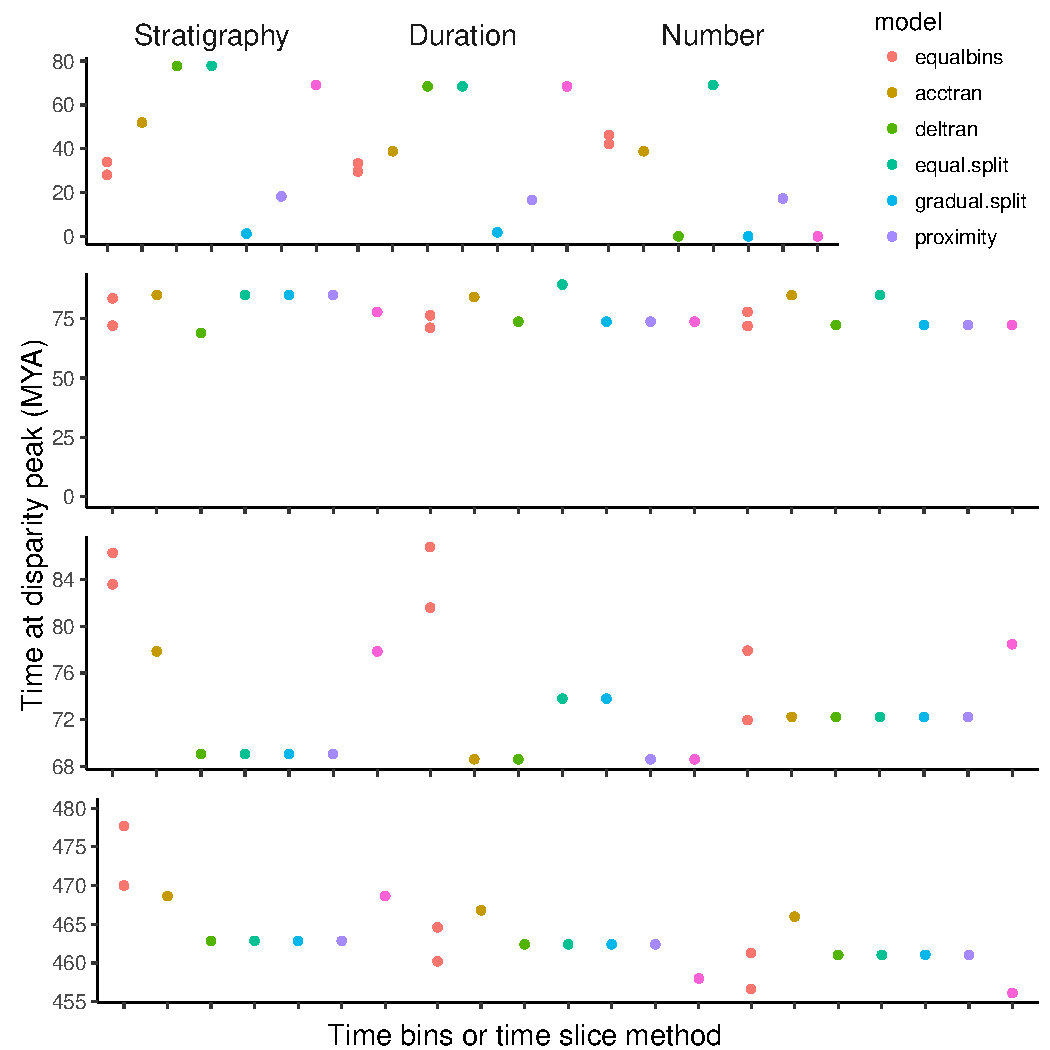
\includegraphics[width=1\linewidth, height=1\textheight, keepaspectratio]{figures/fig-peaks-age-appendix.pdf}
    \caption[Timing of peak disparity for four example datasets.]
    {Median bootstrapped disparities were calculated using time binning and time-slicing approaches. 
    Stratigraphy uses unequal time bins or non-equidistant slices, where the width of the bin, or the interval between slices, is equivalent to stratigraphic ages. 
    Duration uses equal time bins or equidistant slices, where the width of the bin, or the interval between slices, is the average duration of stratigraphic ages in the time frame of the dataset. 
    Number uses equal time bins or equidistant slices, where the number of bins, or the number of slices, is the average number of stratigraphic ages in the time frame of the dataset. 
    For time bins there are two points indicating the maximum and minimum ages of the time bin within which peak disparities appeared.
    The four dataset names are on the first plot for each dataset (Table 1).}
    \label{figure:peak3}
  \end{figure}

% Extinction figures


\end{document}